On April 26, 1920, Harlow Shapley and Heber Curtis took the stage at the
Smithsonian National Museum of History to debate each other on a topic of of
seemingly only academic interest: the nature of so-called ``Spiral Nebulae''.
The two eminent astronomers argued whether these nebulae were contained within
the Milky Way.  The implication if they lived within the Galaxy was that the
Galaxy was the Universe.  If they were not, the universe was far vaster than
many imagined.  This academic debate, like the Papal disagreement with Galileo
three hundred years earlier, was poised to reshape our understanding of the
vastness of the cosmos, and our insignificant place within it.

Today, nearly a century later, we no longer refer to these objects as ``Spiral
Nebulae'', but instead give them the name first reserved only for our own:
Galaxies.  Our Milky Way is but one of trillions of galaxies in the universe,
filling a volume that stretches out thousands of Megaparsecs in space and
billions of years in time.  These galaxies contain nearly all of the stars and
planets in the universe, much of the universe's gas, and are the places where
the former are constructed from the latter.

Galaxies within our universe are all made up of a common set of components.  The
most obvious component, and the one we can actually observe here in our own
galaxy with the naked eye, is the stellar component.  Galaxies are the sites in
which stars form, and those luminous stars are the most easily observed piece of
the galactic pie.  Those stars are formed out of a gaseous
interstellar medium (ISM).  This ISM is, in most galaxies, multiphase,
containing molecular gas, typically with densities $>100\;\rm{cm^{-3}}$ and
temperatures below $100\;\rm{K}$; a cold neutral medium with slightly higher
temperatures and lower densities; a warm neutral/ionized medium, with
temperatures around $10^4\;\rm{K}$; and a hot ionized medium with temperatures
$>10^5\;\rm{K}$.  All of this is surrounded by a hot ionized circumgalactic
medium that gives way to the hot coronal gas filling a dark matter halo much
larger than the galaxy disc itself.

Each of these baryonic components have been observed by a wide array of
telescopes both on earth and in orbit.  The dark matter that fills the galactic
halo must be observed indirectly: through the increased rotational velocity it
imparts on the stars and gas in the disc, and through gravitational lensing of
background objects.  While these observations are extremely powerful tools for
understanding how galaxies function in the present and how they have formed over
time, the immense timescales involved in both internal processes and in the
evolution of the galaxy itself make it impossible to watch them take place in
any single object.  To do this, and to test our theoretical models of how
galaxies evolve, requires numerical modeling.

Numerical modeling of galaxies is a difficult problem, as it involves processes
that take place over scales (both spatial and temporal) that span many orders of
magnitude.  This means that simulations will always be unable to resolve at
least some fraction of the physics taking place within the galaxy.  For this,
carefully designed ``sub-grid'' models are required to include the macroscopic
effects that unresolvable microscopic processes yield.  In this thesis, I
present a new sub-grid model for the feedback from massive stars (Chapter 2).  I
use that model to investigate how this feedback can regulate the formation of
stars within galaxies (Chapters 3 and 4), and finally show how this same
feedback is unneeded to produce galaxies that match the observations of
\citet{McGaugh2016} (Chapter 5).  I conclude with a summary of these results,
their implications, and some potential future directions for study in Chapter 6.

\section{The Cosmological Context of Galaxy Formation}
The modern picture of galaxy formation sits within the context of a $\Lambda$
Cold Dark Matter  ($\Lambda CDM$) cosmology.  This is a universe which has a no
curvature, the majority of its mass-energy in a cosmological constant $\Lambda$,
and most of its matter in a collisionless form (Dark matter).  Roughly $5\%$ of
the universe exists as baryons, which began as a mostly isothermal gas of
hydrogen and helium.  All of this began roughly $13.8$ billion years ago, with
the universe emerging from a state of infinite temperature and density,
expanding to form what we see today.  The primordial elemental abundances, with
$\sim4/5$ of the universe's baryons in hydrogen, and the remainder in helium,
was established just a few minutes after the big bang, during a brief period
called ``Big Bang Nucleosynthesis''.  The remaining elements of the periodic
table have been formed through stellar nucleosynthesis, through fusion in the
cores of stars and in energetic processes that take place during supernovae.

Much of what we know about the cosmology of our universe comes from observations
of the first light to escape the universe as it became optically thin and thus
transparent.  Prior to a redshift of $z=1100$, the universe had a high enough
ionization fraction that the mean free path for photons was short, making all of
space effectively opaque.  Once the universe became cool enough that hydrogen
became neutral, the optical depth was now low enough that photons could
free-stream, decoupled from baryons.  This ultraviolet light we observe today,
redshifted to microwaves with a temperature just $\sim2.7\;\rm{K}$.  When the
power spectrum of this radiation is measured, features in that spectrum can be
used to determine the components of the universe, as well as the spectrum of
density perturbations that will eventually form galaxies.

The formation of galaxies within the universe began with the gravitational
collapse of small, linear density perturbations that were likely seeded by
quantum fluctuations amplified by inflation.  These perturbations grow through
gravitational collapse.  Until $z\sim1100$, only dark matter perturbations were
able to grow.  Prior to this, baryons were coupled to photons, causing density
perturbations to simply oscillate as stable sound waves.  This early collapse of
matter meant that when decoupling occurred at $z\sim1100$, baryons were able to
collapse into the deeper potential wells grown out of dark-matter density
perturbations.  These overdensities expand slower that the surrounding medium,
as they experience a drag from their own self-gravity.  Eventually, these
regions stop expanding altogether and begin collapsing at the turnaround time
$t_{turn}$, and virialize at $2t_{turn}$. The first galaxies likely began to
form around $z\sim20-50$.


The perturbation spectrum that forms the structure in which galaxies begins to
form is essentially a Gaussian random field, which \citet{Press1974} were able
to show produces a halo mass spectrum at a given time with a relatively simple form:
\begin{equation}
    \frac{dn}{dM}(M,t) =
    \sqrt{\frac{2}{\pi}}\frac{\rho_0\delta_c(t)}{M^2\sigma(M)} 
    \left\lvert\frac{d\ln{\sigma}}{d\ln{M}}\right\rvert
    \exp{\left[-\frac{\delta^2_c(t)}{2\sigma^2(M)}\right]}
\end{equation}
In this equation, $\rho_0$ is the mean density of the universe, and $\delta_c(t)$
is the critical overdensity for collapse at a given time $t$.  The mass variance
spectrum, $\sigma^2(M)$ can be determined observationally using the CMB power
spectrum.  This function gives a distribution of masses for the dark matter
halos that galaxies will begin to form within.  As these halos collapse,
gravitational torques from their surroundings will impart torques on them,
causing each galaxy to have angular momentum that will be conserved as their
baryonic components collapse and form a disc.

The collapse of baryons within the will depend strongly on whether the
post-virialized gas can cool radiatively.  As gas accretes onto a halo with
overdensity $\Delta$ it passes through a shock that raises its temperature to
the virial temperature:
\begin{equation}
    T_{virial} = \frac{2}{3}\frac{G\mu m_H}{k_B}\left({\frac{4\pi\rho_0\Delta
    M^2}{3}}\right)^{1/3}
\end{equation}
This means that more massive halos have larger virial temperatures, and,
depending on the mode of radiative cooling (atomic cooling from primordial
hydrogen, molecular hydrogen cooling, or cooling through metal lines), this may
give cooling times shorter than the current age of the universe.  These halos 
are the ones in which galaxy formation may begin, as their hot gaseous halos may
can collapse to form a disk, with a cold ISM where star formation can occur.

\begin{figure}
    \includegraphics[width=0.7\textwidth]{mass_function.eps}
    \caption[Galaxy mass function]{The observed mass function for galaxies in
    the nearby universe does not match the mass function for dark matter halos
    given in equation 1, scaled by the baryon fraction.  This tells us that
    there are additional physical processes involved in the formation of
    galaxies within their dark matter halos.  The most likely candidate for
    this is feedback from stars and black holes.  Of particular interest is the
    peak in star formation efficiency near $M_{200}=10^{12}M_\odot$.
    \textit{Image credit: Adapted from figure 1 in \citet{Ferrero2012}}}.
\end{figure}

This is of course all highly idealized, simple models for the earliest stages of
galaxy formation.  Each of these halos will begin to undergo mergers and
interactions with each other that can strip stars and gas through tidal and ram
pressure forces.  Inside each of these halos, the process of disc collapse, star
formation, and feedback from those stars involves the complex interplay of
radiation, hydrodynamics, magnetic fields, and gravity on length scales as much
as $10^{11}$ times smaller than the virial radius.  None of this physics is
simple enough to be captured by these sorts of analytic models, and so numerical
simulations have become a keystone for galaxy formation research.

\section{Numerical Simulations of Galaxies}
Simulations of galaxies actually predate {\it numerical} simulations of
galaxies.  \citet{Holmberg1941} presented, as the author termed it, a ``new
integration procedure'' that was arguably the first attempt to simulate the
evolution of galaxy.  By relying on the fact that light flux, just as gravity,
scales as $r^{-2}$, Holmberg was able to construct a simulated galaxy disc out
of light bulbs, and then using photocells to measure the flux at each bulb's
position, repositioned the bulbs using the forces ``simulated'' by the
light-measuring process.  This allowed him to painstakingly trace the tidal
interactions of passing galaxies as they fell into a galaxy cluster.

In the intervening 75 years, we have migrated to much less labor-intensive
simulations, relying on the constantly growing power of digital computers.  As
Gordon Moore first observed in 1965, the processing power of computers has been
continuously growing at an exponential rate for more than half a century.  This
has meant that, even without advances in numerical methods and algorithm design,
the ability of simulators today to model a system in high resolution is
monumentally greater than just 10 years ago.  

\begin{figure}
    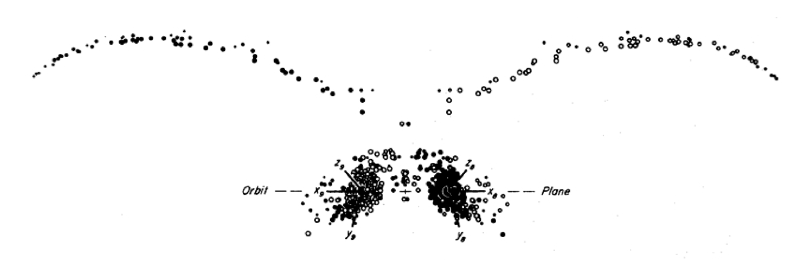
\includegraphics[width=0.8\textwidth]{Toomre.eps}
    \includegraphics[width=0.8\textwidth]{Antennae.eps}
    \caption[Early simulation of Antennae Galaxies]{The simulations of
    \citet{Toomre1972} showed how the kinematics of galaxy mergers can produce
    the variety of tidal structures seen in objects like the Antennae galaxies.
    The top image shows the result of one of the \citet{Toomre1972} simulations.
    \textit{Image credit: Adapted from figure 23 of \citet{Toomre1972}}
    The bottom image shows an observation of the actual object itself, the
    Antennae galaxies NGC 4038/4039. \textit{Image credit: NOAO/AURA/NSF, B.
    Twardy, B. Twardy, and A. Block (NOAO)}}
\end{figure}

The earliest numerical simulations of galaxy formation focused on the
effects of gravity alone.  A classic example of this are the simulations
presented in \citet{Toomre1972}, which showed that the irregular structures seen
in galaxies like NGC 4676 (``The Mice'') or NGC4038/4039 (``The Antennae
Galaxies'') are the results of major mergers between two disc galaxies.  These
simulations used discs composed of a mere 120 test particles, and ignored the
effects of self-gravity between these particles.  Despite the crudeness of these
simulations, these simulations definitively showed that galactic bridges and
tails could be formed by the tidal interactions of two passing/merging galaxies.
The IBM 360/95 that \citet{Toomre1972} (with an inflation-adjusted purchase
price in the millions of dollars) used for their simulations was capable of
5.5 million instructions per second, roughly $0.2\%$ the speed of the 35\$
Raspberry Pi 3 available today.

Modern galaxy simulations do far more than merely integrate the equations of
motion for a few hundred test particles in a gravitational field.  Today, state
of the art simulations will track gravity (including self-gravity) for stars,
gas, and dark matter; evolve Euler's equations for the hydrodynamics of gaseous
baryons; include models for radiative cooling of gas that allow for cooling from
both hydrogen and metal lines; form stars from dense gas; and include models for
feedback from massive stars and black holes.  Often, simulations will also
include treatments for radiative transfer and magneto-hydrodynamics as well.
Hydrodynamical solvers usually come in one of two classes: Eulerian or
Lagrangian.  Eulerian methods discretize space, breaking a simulation volume
into a grid of cells that each contains a number of scalar and vector quantities
that are advected according to the solver scheme.  Lagrangian methods instead
discretize mass, breaking the gaseous volume into discrete points, each of which
is moved to advect the quantities it contains, with smoothing functions used to
interpolate values in between particles.  Recently, new methods have begin to
hybridize features of each of these classes as well. Gravity is typically solved
using algorithms designed to minimize the workload that would be needed for a
direct summation of each particle or grid cell ($\mathcal{O}(N^2)$ for N grid
cells/particles).  Most codes use a tree-like or spectral algorithm to reduce
the cost to $\mathcal{O}(N\log{N})$, though a handful are beginning to adopt the
even faster Fast Multipole Method to reduce gravity calculation cost to
$\mathcal{O}(N)$.

In simulations of galaxies, the formation and deaths of individual stars are
typically unresolvable (in fact, this is currently true even for simulations of
molecular clouds).  This means that the formation of stars must be handled by
sub-grid approximations of the complex physics taking place at the sites of star
formation.  The simplest and most straight forward model is to simply assume
that gas will form stars at some fraction of the local free-fall time.  This leads
to a star formation rate that scales like $\dot \rho_* = c_* \rho_{gas}^{1/2}$,
where the single parameter $c_*$ is intended to capture the unresolved
efficiency of star formation at small scales.  

Modern galaxy simulations also now use a variety of strategies for judiciously
applying computational power where it is most needed.  Eulerian methods will
commonly use \textit{Adaptive Mesh Refinement} to increase resolution in regions of
interest (typically where gas is densest).  Lagrangian methods automatically do
this, as a denser region definitionally must contain more particles.  Beyond the
choice of algorithms, the choice of what type of simulation to set up in the
initial conditions is also important.  To study large populations of galaxies,
along with large-scale structure, large-volume cosmological boxes with
$>>10^4\;\rm{Mpc^3}$, but with spatial resolutions $\sim \rm{kpc}$ are used.
Studying how individual galaxies form is typically done with cosmological zoom
simulations, where a comparatively cheap dark-matter only simulation is first
run to select a region of interest, which is then resimulated with higher
resolution and baryonic physics included. Zoom-in simulations can typically
achieve an order of magnitude or better resolution than full cosmological boxes.
Isolated galaxy disc simulations cannot show how galaxies form in a cosmological
environment, but can be run with $\sim \rm{pc}$ resolution to study closely how
internal processes within a galaxy take place.

\section{The Importance of Feedback}
Simple analytic models for galaxy formation began with a universal picture of
their formation:  density perturbations that, over time, collapse under their
own self-gravity.  It is tempting to assume that this process dominates at all
scales of interest, as clearly stars form through the gravitational collapse of
gas clouds within the ISM (which themselves may form through their own
self-gravity).  This leads to a catastrophe at nearly all scales.  If gravity
is unopposed in star and galaxy formation, the timescales involved would scale
like the freefall time:
\begin{equation}
    t_{ff} = \sqrt{3\pi/32G\rho}
\end{equation}
The observed timescales for star and galaxy formation are much longer than this.
For galaxies, this predicts a complete conversion of gas to stars in $t_{ff} <<
t_{Hubble}$, which would mean the universe today would contain far more stars
than it does, and no actively star-forming galaxies.

We now know that galaxy and star formation is not a one
way process of gravitational collapse.  A number of internal processes
(``feedback'') within galaxies can liberate energy greater than the
gravitational binding energy of molecular clouds (and indeed even comparable to
the binding energy of the entire halo).  Early simulations that omitted
these feedback processes found that gas rapidly collapsed into the smallest
halos at high redshift, wildly overproducing stars in small galaxies at
high redshift (the ``cooling catastrophe'').  Galaxies like our own develop
unrealistically compact morphologies.  Simulations of individual molecular
clouds develop star formation rates an order of magnitude too high.  Aside from
establishing a number of observed galaxy properties, there are a observations of
feedback processes taking place.  Fast, massive outflows have been observed
leaving the discs of starburst galaxies and quasar host galaxies.  These
outflows must be powered by feedback.

\begin{figure}
    \includegraphics[width=0.8\textwidth]{M82.eps}
    \caption[Massive outflows in M82]{The evidence for feedback is no clearer
    than here in the Cigar Galaxy, M82.  The Hubble Space Telescope reveals
    massive outflows of hot ionized gas through the red $H\alpha$ emission seen
    as gas is blasted out of the galaxy in a bipolar flow. \textit{Image credit:
    NASA, ESA and the Hubble Heritage Team STScI/AURA}}
\end{figure}

Feedback energy may come from a number of sources.  The two primary sources are
massive stars and supermassive black holes (SMBHs).  Massive stars ($M>5M_\odot$)
live short, violent lives.  During their lives, they will drive fast
$v>1000\;\rm{km/s}$ stellar winds, and heat their surrounding gas with UV
radiation.  At the end of their lives $4-30\;\rm{Myr}$ later, these stars die in
extremely energetic core-collapse supernovae, liberating $\sim10^{51}\;\rm{erg}$.
This energy imparts heat and momentum to the surrounding ISM, and can accelerate
cosmic rays in the shocks that are driven.  In galaxies with actively growing
SMBHs, the accretion disc that forms as gas funnels into the black hole can
reach temperatures exceeding $10^9\;\rm{K}$ through viscous heating.  This
makes these accretion discs some of the most luminous objects in the universe,
and can heat the gas that surrounds the galaxy to choke off the accretion of new
material to form stars.

On the galactic scale, feedback regulates star formation in two primary ways.
Energy and momentum deposited into the ISM can heat and disrupt the cool clouds
of gas which form stars.  If that feedback is vigorous enough, this gas can
actually be ejected from the disc into the circum-galactic medium (CGM).  This
limits star formation by simply removing the fuel for the process.  Both of
these processes must be happening to explain observations of low star
formation efficiencies in molecular clouds, outflowing gas, a metal-polluted
intergalactic medium, and the low bulge fraction in star forming galaxies.

The greatest difficulty with including the effects of feedback in simulations of
galaxy evolution is the combination of extreme energy gradients in a relatively
small mass/volume.  Without overwhelmingly high resolution, hot feedback gas
will be numerically mixed with cold ISM, often resulting in gas with
temperatures of $\sim10^5\;\rm{K}$, at the peak of the ISM cooling curve where
cooling times are extremely short.  This results in feedback energy being
completely lost due to radiative cooling.  Indeed, as \citet{Thacker2000}
showed, how feedback energy is deposited into the ISM has a huge impact on
whether that feedback has any impact.  This problem has been tackled using a few
different strategies.  Since overcooling is the problem, many models have
attacked this directly by either temporarily disabling cooling
\citep{Stinson2006} or depositing feedback energy into a second, nonthermal
energy component \citep{Agertz2013}.  While this does limit radiative losses, it
produces gas that exists in an unphysical region of the $\rho-T$ phase diagram,
which may not have the correct entropy to escape buoyantly.  It also has the
potential to introduce an \textit{undercooling} problem as resolution becomes
higher and feedback-heated gas becomes resolvable.  Alternatively, energy may be
injected not as heat, but as momentum, which naturally does not cool.
Unfortunately, this adds the additional complexity of momentum cancellation (how
to treat neighbouring stars/clusters?), and if this momentum results in strong
shocks, these shocks will convert the momentum right back into thermal energy
that can radiate away the feedback energy the model is designed to preserve.
This often means kinetic/momentum feedback models must be combined with
hydrodynamic decoupling that renders feedback-heated gas into a form that does
not interact with the surrounding ISM.  Naturally, this makes outflow properties
strongly influenced by numerical choices.  

A third choice is to stochastically deposit feedback energy only when enough
energy is available to raise gas temperatures high enough for cooling times to
be short \citep{DallaVecchia2012,Crain2015}.  In these models, supernovae events
are effectively grouped together, somewhat decoupling feedback from star
formation.  The choice of temperature to heat gas to is a purely numerical
parameter, and can dramatically change the effectiveness of these models.
Finally, some \citep{Springel2010} attempt to directly address the unphysical
numerical mixing of hot and cold gas by separating the two phases and tracking
each component separately.  This completely solves the overcooling problem, and
allows the two components to cool radiatively.   Unfortunately, it also means
that cold star-forming gas is permanently coupled to hot feedback-heated gas:
effectively making the ISM an anchor holding down potential hot outflows.  This
means these multiphase models have to be coupled with parameterized models to
capture outflows.  Often, these simple models simply choose a fraction of
feedback energy to be deposited as kinetic ``kicks'' to a some gas particles.
Like other kinetic feedback models, this is frequently combined with
hydrodynamical decouplings.

All of these models attempt to solve the problem of overcooling with unphysical
approximations: disabled cooling, hydrodynamic decoupling, and stochastic
deposition of feedback energy.  These choices make it difficult to understand
what details of simulated galaxy evolution are a result of these numerical free
parameters, as opposed to the actual physics of feedback-regulated star
formation and outflows.  What is needed is a model that captures the effects of
feedback while matching as closely as possible the actual physical processes
involved below the resolution scale.

\section{Superbubble Feedback}
The formation of massive stars takes place mostly in clusters of $10^4$ or more
stars.  This means that the supernovae of these stars can be treated not as
individual dumps of $10^{51}\;\rm{erg/SN}$, but instead as a luminosity of
$10^{38}\;\rm{\frac{erg}{s \cdot M_\odot}}$.  This allows us to use stellar wind
models like \citet{Weaver1977} to study the evolution of superbubbles driven by
clustered supernovae.  Each individual supernovae's eject thermalizes in a small
region within the center of the bubble, and the resulting hot gas drives a shock
that sweeps up the surrounding ISM.  In a short time, the swept-up ISM can
efficiently radiatively cool, resulting in a thin, cold shell surrounding a hot
bubble.

The evolution of these superbubbles was studied in detail in \citet{MacLow1988}.
A key insight was that the hot bubble would evaporate the cold shell through
thermal conduction.  In a hot ionized plasma, electrons are able to penetrate
temperature gradients and deposit energy within cooler material, and via charge
conservation, establishing a mass flux against the temperature gradient.  This
evaporation means that the hot bubble with radius $R$ gains mass at a rate of:
\begin{equation}
    \frac{{\rm d }M_b}{{\rm d}t} = \frac{16\pi\mu}{25k_B} CT^{5/2}R
\end{equation}
Where $C=6\times10^{-7}\;\rm{erg\;s^{-1}\;cm^{-1}\;K^{7/2}}$, and $\mu$ is the
mean molecular weight of the gas in the bubble.  As the cold, evaporated
material acts to cool the hot bubble, this makes the bubble's interior
temperature self-regulating: higher temperature give higher mass flux, cooling
the bubble.

\citet{DallaVecchia2012} showed that the temperature of feedback-heated gas can
ultimately determine its effectiveness in driving outflows and regulating star
formation, even with constant feedback energy.  The self-regulating temperature
of superbubbles suggests that nature has a mechanism for setting
this temperature: thermal evaporation.
\bibliographystyle{mnras}
\bibliography{library}
